%%%%%%%%%%%%  Generated using docx2latex.pythonanywhere.com  %%%%%%%%%%%%%%


\documentclass[a4paper,12pt]{report}

% Other options in place of 'report' are 1)article 2)book 3)letter
% Other options in place of 'a4paper' are 1)a5paper 2)b5paper 3)letterpaper 4)legalpaper 5)executivepaper


 %%%%%%%%%%%%  Include Packages  %%%%%%%%%%%%%%


\usepackage{amsmath}
\usepackage{latexsym}
\usepackage{amsfonts}
\usepackage{amssymb}
\usepackage{graphicx}
\usepackage{txfonts}
\usepackage{wasysym}
\usepackage{enumitem}
\usepackage{adjustbox}
\usepackage{ragged2e}
\usepackage{tabularx}
\usepackage{changepage}
\usepackage{setspace}
\usepackage{hhline}
\usepackage{multicol}
\usepackage{float}
\usepackage{multirow}
\usepackage{makecell}
\usepackage{fancyhdr}
\usepackage[toc,page]{appendix}
\usepackage[utf8]{inputenc}
\usepackage[T1]{fontenc}
\usepackage{hyperref}


 %%%%%%%%%%%%  Define Colors For Hyperlinks  %%%%%%%%%%%%%%


\hypersetup{
colorlinks=true,
linkcolor=blue,
filecolor=magenta,
urlcolor=cyan,
}
\urlstyle{same}


 %%%%%%%%%%%%  Set Depths for Sections  %%%%%%%%%%%%%%

% 1) Section
% 1.1) SubSection
% 1.1.1) SubSubSection
% 1.1.1.1) Paragraph
% 1.1.1.1.1) Subparagraph


\setcounter{tocdepth}{5}
\setcounter{secnumdepth}{5}


 %%%%%%%%%%%%  Set Page Margins  %%%%%%%%%%%%%%


\usepackage[a4paper,bindingoffset=0.2in,headsep=0.5cm,left=1.0in,right=1.0in,bottom=2cm,top=3cm,headheight=3cm]{geometry}
\everymath{\displaystyle}


 %%%%%%%%%%%%  Set Depths for Nested Lists created by \begin{enumerate}  %%%%%%%%%%%%%%


\setlistdepth{9}
\newlist{myEnumerate}{enumerate}{9}
	\setlist[myEnumerate,1]{label=\arabic*)}
	\setlist[myEnumerate,2]{label=\alph*)}
	\setlist[myEnumerate,3]{label=(\roman*)}
	\setlist[myEnumerate,4]{label=(\arabic*)}
	\setlist[myEnumerate,5]{label=(\Alph*)}
	\setlist[myEnumerate,6]{label=(\Roman*)}
	\setlist[myEnumerate,7]{label=\arabic*}
	\setlist[myEnumerate,8]{label=\alph*}
	\setlist[myEnumerate,9]{label=\roman*}

\renewlist{itemize}{itemize}{9}
	\setlist[itemize]{label=$\cdot$}
	\setlist[itemize,1]{label=\textbullet}
	\setlist[itemize,2]{label=$\circ$}
	\setlist[itemize,3]{label=$\ast$}
	\setlist[itemize,4]{label=$\dagger$}
	\setlist[itemize,5]{label=$\triangleright$}
	\setlist[itemize,6]{label=$\bigstar$}
	\setlist[itemize,7]{label=$\blacklozenge$}
	\setlist[itemize,8]{label=$\prime$}



 %%%%%%%%%%%%  Header here  %%%%%%%%%%%%%%


\pagestyle{fancy}
\fancyhf{}
\chead{\begin{flushright}\chapter{  }
\end{flushright} \par
\noindent 


 %%%%%%%%%%%%  Figure/Image No:1 here %%%%%%%%%%%%%%


\begin{figure}[H]
\begin{center}

\includegraphics[width=6.47in,height=0.11in]{./uploads_new/Lab_2.docx_DIR/media/image2.png}
\end{center}
\end{figure}


 %%%%%%%%%%%%  Figure/Image No:1 Ends Here %%%%%%%%%%%%%%


\vspace{12pt}
}


 %%%%%%%%%%%%  Footer here  %%%%%%%%%%%%%%




 %%%%%%%%%%%%  Print Page Numbers  %%%%%%%%%%%%%%


\rfoot{\thepage}


 %%%%%%%%%%%%  This sets linespacing (verticle gap between Lines) Default=1 %%%%%%%%%%%%%%


\setstretch{1.2}


 %%%%%%%%%%%%  Document Code starts here %%%%%%%%%%%%%%


\begin{document}
\sloppy
\subsection*{ }
 \par
\noindent 


 %%%%%%%%%%%%  Figure/Image No:2 here %%%%%%%%%%%%%%


\begin{figure}[H]
\begin{center}

\includegraphics[width=6.46in,height=4.31in]{./uploads_new/Lab_2.docx_DIR/media/image8.jpg}
\end{center}
\end{figure}


 %%%%%%%%%%%%  Figure/Image No:2 Ends Here %%%%%%%%%%%%%%


\vspace{12pt}
\noindent 
\appendix
\textit{\textbf{\Huge Gourmet Restaurant Management\\ Systems}} \\ \\
\textit{ \emph{28.08.2017}}
 \par
\noindent 
 \par
\noindent 
{\fontsize{18pt}{18pt}\selectfont \textbf{─} \\} \par
\noindent 
\newpage
{\fontsize{16pt}{16pt}\selectfont \textbf{Team Members} \\} \par
\noindent 
{\fontsize{14pt}{14pt}\selectfont Tumelo Moloi - 816926(GL) \\} \par
\noindent 
{\fontsize{14pt}{14pt}\selectfont Samkelisiwe Mhlanga - 937608  \\} \par
\noindent 
{\fontsize{14pt}{14pt}\selectfont Ishmael Sibisi - 915702 \\} \par
\noindent 
{\fontsize{14pt}{14pt}\selectfont Lesego~Seritili - 722957   \\} \par
\noindent 
\section*{Overview}
 \par
\noindent 
Our~client  Marthinus Ferreira is requesting the implementation of custom tailored restaurant software management system to run on a PC server (or on cloud computing service) for his restaurant \textit{DW Eleven}.  \par
\noindent 
The system runs a back-end service which manages all the essential databases, e.g., recipes for dishes, customers and customer orders, stocks of ingredients for the dishes, employees - part-time and full-time hired waiters/waitresses, managers, suppliers of stocks, etc. The front-end services feature interfaces for interacting with the management systems. \par
\noindent 
\section*{Goals}
 \par
\noindent 
Customers: \par
\noindent 
Customers can make orders and reservations to be picked up for take-away, dine-in, home delivery, etc. A unique feature of the gourmet restaurant is that orders may include special request to modify the content of the dish, e.g., no-salt, no-sugar, etc. The possible devices for interacting with the system include PCs (desktops), Laptops, tablets, mobile-phones, etc.  \par
\noindent 
Restaurant Manager:  \par
\noindent 
The manager interacts with the system to manage:  \par
\begin{myEnumerate}
\item Stock Inventory \par
\item Recipe/Menu planning \par
\item Reservations \par
\item Dish/Food costs \par
\item Customer database  \par
\item Track delivery \par
\item Accounting/Financial Administration \par
\item Waiters’/Waitresses’ duties, off-days, leaves, etc. \par
\item Generation of reports - Analytics \par
\item Special events \end{myEnumerate}
 \par
\vspace{12pt}
\vspace{12pt}
\noindent 
\section*{Development Cycle choice}
 \par
\noindent 
Our~team~will~be~implementing~the agile development cycle. Upon further investigations to see the fitting development for our system, the  Rapid Application Development (RAD) and Dynamic Systems Development Method (DSDM)  were not fitting team, we decided to use the SCRUM approach as our team is comprised of 4 members and easily assigning the group leader as the scrum master who will be responsible for setting the sprint dates. The project will be completed using incremental loads instead of implementing it all at once, hence, SCRUM also taking into account philosophies from LEAN and Kanban, but fundamentally sticking to SCRUM.     \par
\vspace{12pt}
\noindent 
\section*{System Architecture}
 \par
\subsection*{Hardware & Software architecture}
 \par


 %%%%%%%%%%%%  Figure/Image No:3 here %%%%%%%%%%%%%%


\begin{figure}[H]
\begin{center}
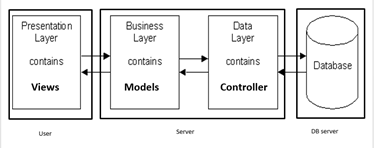
\includegraphics[width=6.5in,height=2.57in]{./uploads_new/Lab_2.docx_DIR/media/image7.png}
\end{center}
\end{figure}


\vspace{12pt}
The team will be using a three tier system architecture. All of the software that will be interacting with the system will be listed on the front-back end section.  \par
\vspace{12pt}
\section*{Front end services for the system   }
\par
\begin{itemize}
\item Nodejs \par
\item Reactjs \par
\item Ionicjs \par
\item Electronjs \par
\item scss/css3 \par
\item HTML5 \par
\section*{Back end services for the system }
\par
\begin{itemize}
\item Php \par
\item Mysql \par
\item mongoDB \par
\item graphQL \par
\item Apache Web Server \par
\section*{Supporting tools for the system }
\par
\vspace{12pt}
\item Google Maps API (for Maps and location) \par
\item Facebook/twitter/Instagram APIs (for social media integration)\end{itemize}
 \par
\end{document}
